\begin{figure*}
  \begin{center}
    \begin{tabular}{c}
      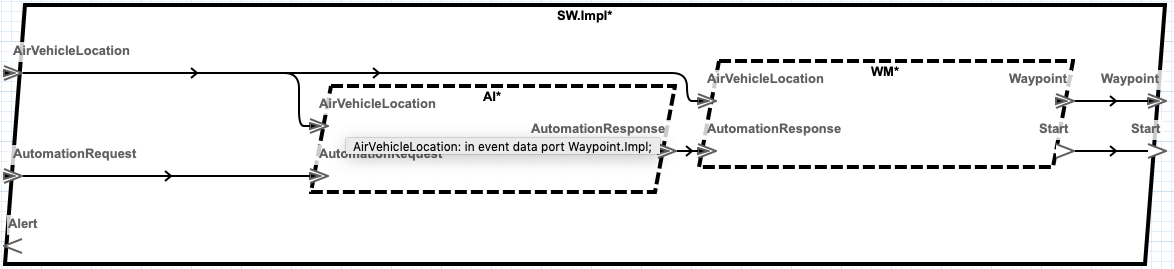
\includegraphics[scale=0.3]{example.png} \\
      (a) \\
      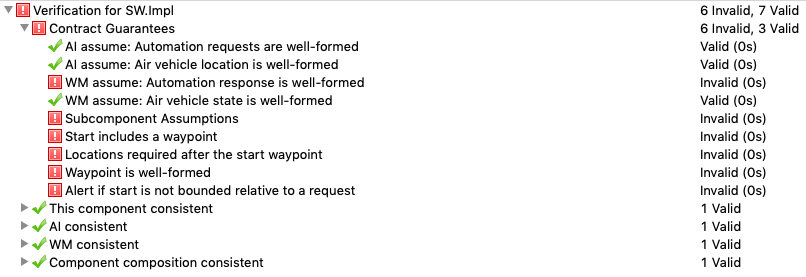
\includegraphics[scale=0.3]{example-certificate.png} \\
      (b)
    \end{tabular}
  \end{center}
\caption{Automated UAV route planning system. (a) Unhardened system. (b) Failure certificate.}
\label{fig:example}
\end{figure*}

\figref{fig:example} is an AADL architectural model of a software system (SW) for route planning and automated control of a UAV. It is loosely based on the system in the case study introduced in Section~\ref{sec:case-study}.  The source for the entire model is found at \cite{repo}. The system receives an automation request that is forwarded to an untrusted third-party route planner (AI).  The route planner decides the flight path of the UAV based on its current position and the requested task. The waypoint manager (WM) receives the mission command as a set of waypoints from the planner and starts the UAV flying the mission, issuing waypoints to the UAV flight controller as the UAV location changes. The waypoint manager is an \emph{as is} legacy component.

The expected behavior of the SW system, and the components in its implementation, are modeled with AGREE contract specifications. The contracts constrain input and state properties of output for component models. AGREE performs model checking on this assume-guarantee system to hierarchically prove that the composite system obeys all contract obligations under all possible finite input streams. 

The initial AGREE contract specifications for the components and the overall system make no assumptions about the integrity of the inputs and outputs. A cyber-vulnerability analysis identifies the potential of the untrusted AI route planner component to behave maliciously. In response, the developer modifies the AGREE specification for the AI route planner to model this ability to behave maliciously as an untrusted component by removing any guarantees about its output.  In other words, the AI output is unconstrained in the AGREE specification, allowing it to take on any value and allowing the AI component to send that value at any time.

The contract specifications for the other components are also updated with the threat analysis information by adding in new requirements to mitigate the identified cyber-vulnerabilities. For example, a designer adds to the specification for the legacy waypoint manager assumptions about its input being \emph{well-formed} since that is no longer known \emph{a priori} as the AI route planner output is unconstrained. The systems designer is also responsible for defining the meaning of ``well-formed''; in this example, it is a predicate checking that the waypoints are within bounded value ranges for latitude, longitude, and altitude, with an additional integrity check on message IDs.

The developer adds two other requirements to the SW AGREE specification related to the cyber-vulnerability analysis.  The first, \emph{Waypoint is well-formed} requires all the waypoints sent to the UAV flight controller to be well-formed (it detects if malformed waypoints are propagated downstream).  The second, \emph{Alert if start is not bounded relative to a request}, requires an automation request to correspond with an automation response either in the same step or within one step (it detects if a mission is being started without a request or if the start is delayed more than one step after a request). The goal of these two requirements is to detect if the untrusted component is trying to prevent the UAV from flying its intended mission or to fly a wrong mission. 

AGREE examines the composition of the new specifications for the implementation in \figref{fig:example}(a) to determine whether it complies with the added cyber requirements, by way of model checking. The output from the model checker is shown in \figref{fig:example}(b). The red exclamation points designate properties that do not hold. Each of these failures comes with a counterexample. The results are not unexpected given the AI route planner's unconstrained behavior and the new assumptions about the wellformedness of the input to the legacy waypoint manager. The counterexample for \emph{Alert if start is not bounded relative to a request} shows a response in the first time step with no matching request, a  clear malicious behavior from the untrusted component.

\begin{figure*}
  \begin{center}
    \begin{tabular}{c}
      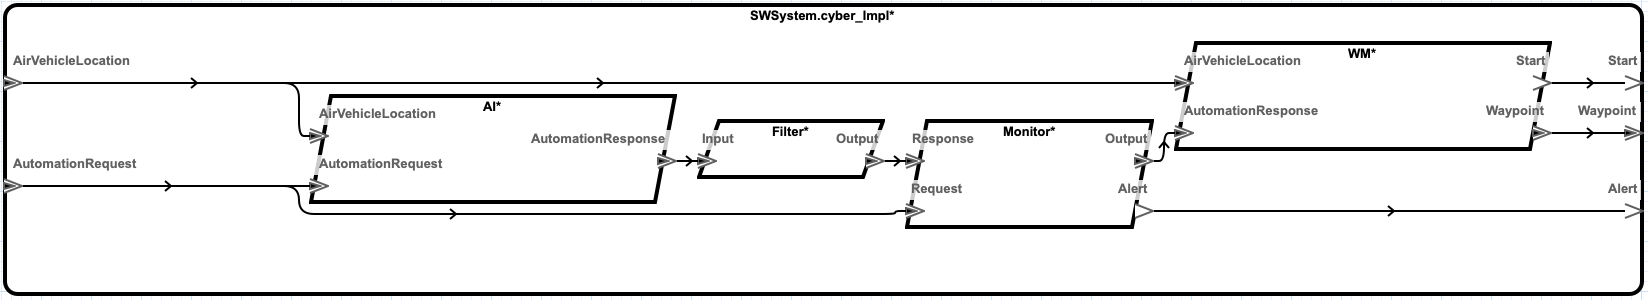
\includegraphics[scale=0.3]{hardened.png} \\
      (a) \\
      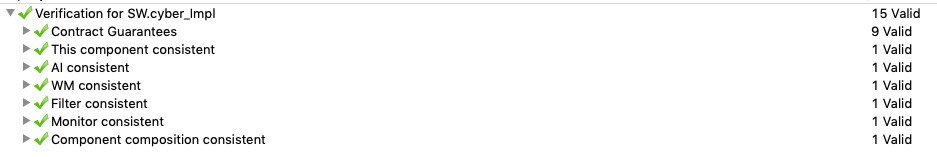
\includegraphics[scale=0.3]{hardened-certificate.png} \\
      (b)
    \end{tabular}
  \end{center}
  \caption{Hardened UAV system. (a) The implementation with high-assurance components. (b) Passing certificate.}
  \label{fig:hardened}
\end{figure*}

The system implementation is cyber-hardened using BriefCASE, which automatically transforms the model by inserting high-assurance components in the form of a filter and a monitor as shown in \figref{fig:hardened}(a). A filter enforces an invariant over each datum in the data stream by not forwarding input to its output if that input violates the filter invariant. The auto-generated AGREE specification states that only well-formed inputs are passed to the output. The system developer must provide this filtering policy, but it is usually based on the existing assumptions made by downstream components that consume the filter output. 

A monitor captures a relation on input data over time and is thus able to reason about temporal properties of that input. A monitor raises an alert if the specified temporal properties are ever violated. The AGREE specification for the monitor in our example states that an automation response can only be generated in conjunction with an automation request; and further,   that response must come with the request or in the next step after the request. As with the filter, the system designer provides the policy, and that policy is based on the existing AGREE specification in the SW system.

The AGREE analysis of the cyber-hardened implementation with the auto-generated high-assurance components is shown in \figref{fig:hardened}(b). Here AGREE provides a proof certificate that the high-assurance components guarantee the correct behavior of the SW implementation in the presence of the considered cyber vulnerabilities from the untrusted AI route planner.

The high-assurance components are automatically synthesized by SPLAT from the AGREE specifications to equivalent models in the CakeML language. CakeML itself provides a complete verified compilation to binaries for several different platforms meaning that the resulting binaries exactly preserve the meaning of the original CakeML code \cite{cakeml}. 

A similar proof is given for the synthesis of the contract model for a high-assurance component to CakeML. A high-assurance component contract has a precise meaning in terms of data streams, and the synthesis exactly preserves that meaning in the generated code. In other words, for any set of input streams that meet the component's contract assumptions, the output streams produced from the synthesized CakeML exactly match the output streams from the high-assurance component's contract. 

Preserving the input/output relationship of streams between the two models lifts the contract verification results to the deployed system. If the contract model verification succeeds, then the meaning of those results hold for the deployed system, given that all other components implement their contracts, an appropriate schedule exists that follows the dependent data-flow, and the communication fabric works as expected.